\documentclass[11pt]{article}
\usepackage[utf8x]{inputenc}
\usepackage[english]{babel}
\usepackage{amstext,amsmath,amssymb,amsfonts,bbm}
\usepackage{graphicx}
\usepackage{epstopdf}
\usepackage{amsthm}
\usepackage{tocvsec2}
\usepackage{enumerate}
\usepackage[many]{tcolorbox}
\usepackage{changepage}
%\usepackage{subcaption}
\usepackage{mathrsfs}
\usepackage{color}
\usepackage{xcolor}
\usepackage{mathtools}
\usepackage{bbm}
\usepackage{braket}
\usepackage{tcolorbox}
\usepackage{natbib}
\usepackage{graphicx}
\definecolor{darkgreen}{rgb}{0.0, 0.2, 0.13}
\definecolor{darkred}{rgb}{0.55, 0.0, 0.0}
\definecolor{myorange}{RGB}{251, 133, 0}
\definecolor{brickred}{rgb}{0.8, 0.25, 0.33}
%\usepackage{refcheck}
\usepackage{titlesec}
\usepackage{dsfont}
\usepackage{slashed}
\usepackage{fullpage}
\usepackage{cite}

\usepackage{float}
%\usepackage[normalem]{ulem}
\usepackage[colorlinks=true,linkcolor=blue,citecolor=brickred,linktocpage=true]{hyperref}
\usepackage{color}
\titleformat*{\section}{\normalsize\bfseries}
\titleformat*{\subsection}{\small\bfseries}
\titleformat*{\subsubsection}{\normalsize\bfseries}
\makeatletter
\renewcommand{\@dotsep}{1000}

\linespread{1.2}

%
\def\Tr{\mathrm{Tr}}
\def\tr{\mathrm{tr}}
\def\De{\mathrm{D}}
\def\de{\mathrm{d}}
\def\i{\mathrm{i}}
\def\k{\mathrm{k}}
\def\mb{\bar{\mu}}
\def\lp{\ell_\text{Pl}}
\def\mp{m_\text{Pl}}
%
\def\A{\mathcal{A}}
\def\B{\mathcal{B}}
\def\C{\mathcal{C}}
\def\D{\mathcal{D}}
\def\E{\mathcal{E}}
\def\F{\mathcal{F}}
\def\G{\mathcal{G}}
\def\H{\mathcal{H}}
\def\I{\mathcal{I}}
\def\J{\mathcal{J}}
\def\K{\mathcal{K}}
\def\L{\mathcal{L}}
\def\M{\mathcal{M}}
\def\N{\mathcal{N}}
\def\O{\mathcal{O}}
\def\Q{\mathcal{Q}}
\def\R{\mathbb{R}}
\def\S{\mathcal{S}}
\def\T{\mathcal{T}}
\def\U{\mathcal{U}}
\def\V{\mathcal{V}}
\def\X{\mathcal{X}}
\def\Y{\mathcal{Y}}
\def\Z{\mathcal{Z}}
\def\t{\boldsymbol{t}}
\def\bo{\boldsymbol{\omega}}

\renewenvironment{thebibliography}[1]
         {\section*{References}\frenchspacing\small
          \begin{list}{[\arabic{enumi}]}
         {\usecounter{enumi}\parsep=2pt\topsep 0pt
         \settowidth{\labelwidth}{[#1]}
         \leftmargin=\labelwidth\advance\leftmargin\labelsep
         \rightmargin=0pt\itemsep=1pt\sloppy}}{\end{list}}


%
\renewcommand{\theequation}{\thesection.\arabic{equation}}\numberwithin{equation}{section}

\newtheorem{remark}{Remark}

\newtheorem{definition}{Definition}

\newtheorem{theorem}{Theorem}

\newtheorem{proposition}{Proposition}

\newtheorem*{proof*}{Proof}


\begin{document}

\title{\Large{\textbf{\sffamily Pattern Recognition and Machine Learning-Exercises}}}
\author{\sffamily Lautaro Amadei}
\date{\small{\textit{
Aix Marseille Univ, Universit\'e de Toulon, CNRS, CPT, Marseille, France}}}

\maketitle

\tableofcontents
\section{Chapter 1. Introduction}

\subsection{Exercise 1.1}
\begin{figure}[bth]
\centering
        {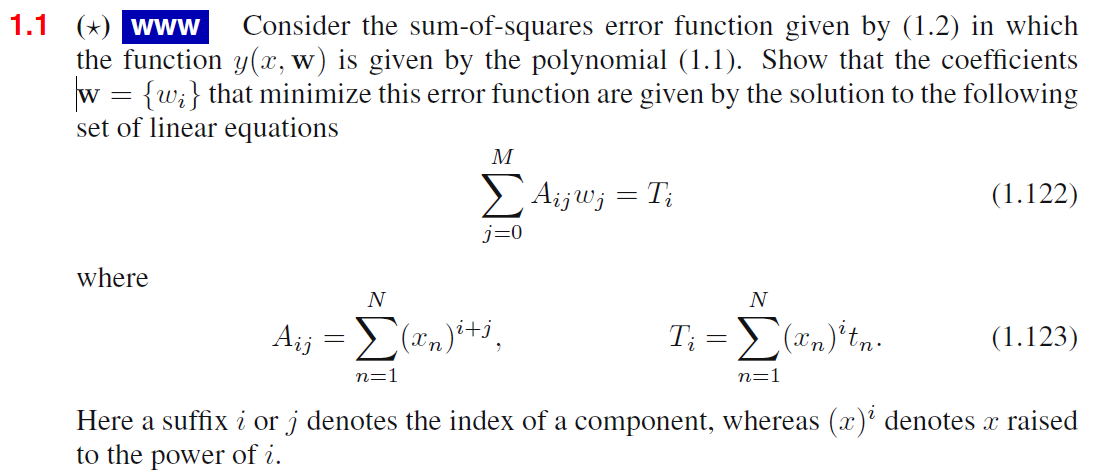
\includegraphics[width=\linewidth]{ex1.png}}
        \caption{Exercise 1.1}
        \label{ex1.1}
\end{figure}


Let us rewrite the error function using Einstein summation notation

\begin{equation}\label{error}
    E(\bo) = \frac{1}{2} \sum_{n = 1}^{N} \left\{ y(x_{n}, \bo) - t_{n} \right\}^2 = \frac{1}{2}\left( y_{a} - t_{a} \right) \left( y^{a} - t^{a} \right)
\end{equation}
where $a= 1, \dots, N$ and $y(\boldsymbol{x}, \bo) = \omega_{\alpha} x^{\alpha}$

We look for the critical points of the function \eqref{error} with respect to $\bo$

\begin{equation}
    \frac{\partial E}{\partial \omega^{\alpha}} = \frac{\partial y_{a}}{\partial \omega^{\alpha}} \left( y^{a} - t^{a} \right).
\end{equation}

Using that 

\begin{equation}
    \frac{\partial y_{a}}{\partial \omega^{\alpha}} = \frac{\partial \omega_{\beta}}{\partial \omega^{\alpha}} x^{\beta}_{a} = \delta_{\beta}^{\alpha} x^{\beta}_{a} = x^{\alpha}_{a},
\end{equation}
and using $y(\boldsymbol{x}, \bo) = \omega_{\alpha} x^{\alpha}$ we obtain:

\begin{equation}\label{der_error}
    \frac{\partial E}{\partial \omega^{\alpha}} = x^{\alpha}_{a} \left( \omega_{\beta} x^{a \ \beta} - t^{a} \right) = 0
\end{equation}

From \eqref{der_error} we obtain the set of equations

\begin{equation}\label{lin_eq_ss}\boxed{
    x^{\alpha}_{a} x^{a \ \beta} \omega_{\beta} =  x^{\alpha}_{a} t^{a}}.
\end{equation}


Or, using book's notation, we define

\begin{align}
    x_{a}^{\alpha} x^{a \ \beta} &= \sum_{n=1}^{N} (x_{n})^{\alpha + \beta} = A^{\alpha \beta} \\
     x_{a}^{\alpha} t^{a} &= \sum_{n=1}^{N} (x_{n})^{\alpha} t_{n} = T^{\alpha}
\end{align}
 and obtain the equations in \ref{ex1.1}
 
 \begin{equation}
     A^{\alpha \beta} \omega_{\beta} = T^{\alpha} 
 \end{equation}
or, more explicitly

\begin{equation}\boxed{
    \sum_{\beta = 0}^{M} A^{\alpha \beta} \omega_{\beta} = T^{\alpha}}
\end{equation}
for $\alpha = 0, \dots, M$.

\subsection{Exercise 1.2}

\begin{figure}[H]
\centering
        {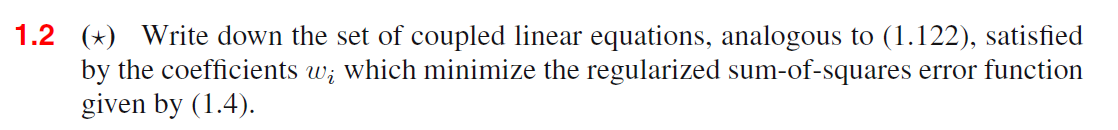
\includegraphics[width=\linewidth]{ex2.png}}
        \caption{Exercise 1.1}\label{ex1.2}
        \label{ex1.2}
\end{figure}

The regularized sum-of-squares error function is given by

\begin{equation}\label{regerror}
    E_{\lambda}(\bo) = \frac{1}{2} \sum_{n = 1}^{N} \left\{ y(x_{n}, \bo) - t_{n} \right\}^2 + \frac{\lambda}{2} |\bo|^{2} = \frac{1}{2}\left( y_{a} - t_{a} \right) \left( y^{a} - t^{a} \right)+ \frac{\lambda}{2} \omega_{\alpha} \omega^{\alpha}
\end{equation}

As before, we look for the critical points of \eqref{regerror}

\begin{equation}
    \frac{\partial E_{\lambda}}{\partial \omega^{\alpha}} = 0 \implies x^{\alpha}_{a} \left( \omega_{\beta} x^{a \ \beta} - t^{a} \right)  + \lambda \omega^{\alpha}= 0,
\end{equation}
and obtain the set of equations

\begin{equation}\boxed{
     \left( x^{\alpha}_{a}  x^{a \ \beta}  + \lambda \delta^{ \alpha \beta 
     } \right)   \omega_{\beta}=x^{\alpha}_{a}  t^{a}}
\end{equation}

Defining 

\begin{align}
    A^{\alpha \beta}_{\lambda} &= x^{\alpha}_{a}  x^{a \ \beta}  + \lambda \delta^{ \alpha \beta 
    } \\
    T^{\alpha} &= x^{\alpha}_{a}  t^{a}
\end{align}
we can write the set of equations in a compact form

\begin{equation}\boxed{
    A^{\alpha \beta}_{\lambda} \omega_{\beta} = T^{\alpha}}
\end{equation}

\subsection{Exercise 1.3}
\begin{figure}[H]
\centering
        {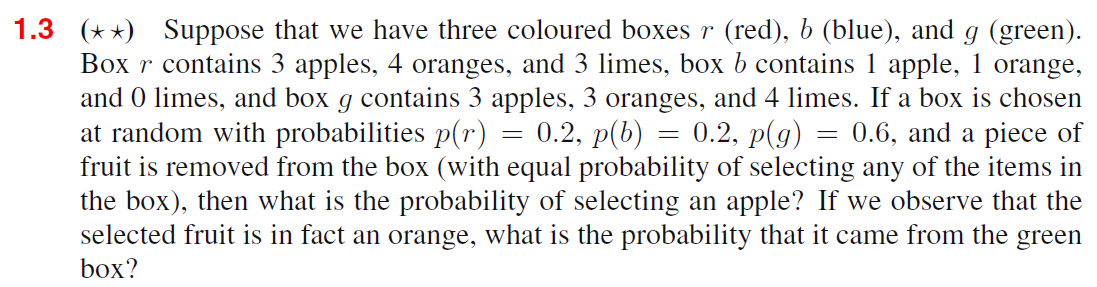
\includegraphics[width=\linewidth]{ex1.3.png}}
        \caption{Exercise 1.2}\label{ex1.2}
        \label{ex1.3}
\end{figure}

We know the posterior probabilities for getting an apple given the color of the box

\begin{align}
    p(a|r) = \frac{3}{10} \\
    p(a|b) = \frac{1}{2} \\
    p(a|g) = \frac{3}{10}
\end{align}
Using Bayes' Theorem we can compute the marginal probability $p(a)$ of getting an apple:

\begin{equation}
    p(a) = p(a|r) p(r) + p(a|b) p(b) + p(a|g) p(g) = \frac{3}{10} \times \frac{1}{5} + \frac{1}{2} \times \frac{1}{5} + \frac{3}{10} \times \frac{3}{5} = \frac{17}{50}
\end{equation}

Now, for computing $p(g|o)$ we use Bayes' theorem

\begin{equation}
    p(g|o) = \frac{p(o|g) p(g)}{p(o)}
\end{equation}

and the marginal probability $p(o)$ of getting an orange

\begin{equation}
    p(o) = p(o|r) p(r) + p(o|b) p(b) + p(o|g) p(g) = \frac{2}{5} \times \frac{1}{5} + \frac{1}{2} \times \frac{1}{5} + \frac{3}{10} \times \frac{3}{5} = \frac{18}{50}.
\end{equation}
Putting everything together, we finally obtain the conditional probability $p(g|o)$

\begin{equation}
    p(g|o) = \frac{3}{10} \frac{3}{5} \frac{50}{8} = \frac{1}{2}.
\end{equation}


\subsection{Exercise 1.5}

\begin{figure}[H]
\centering
        {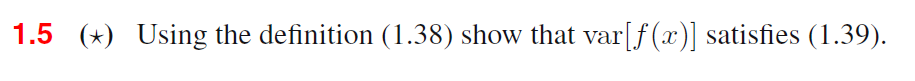
\includegraphics[width=\linewidth]{ex1.5.png}}
        \caption{Exercise 1.5}\label{ex1.5}
        \label{ex1.5}
\end{figure}


\end{document}


